\subsection{\label{subsecWeakDecay}Weakly-decaying Strange Hadrons}

The strange hadrons \kzero, \lmb, \almb, \X, \Ix, \Om\ and \Mo\ are reconstructed at mid-rapidity ($|y|<0.5$)
via their characteristic weak decay topology in the channels~\cite{Patrignani:2016xqp} 

\begin{center}
\begin{tabular*}{0.7\textwidth}{rll@{\extracolsep{2cm}}l}
  \kzero & $\to$ & \pPiplus + \pPiminus & {\footnotesize B.R. = (69.20 $\pm$ 0.05) \%} \\
  \lmb(\almb) & $\to$ & \pProton (\apProton) + \pPiminus (\pPiplus) & {\footnotesize B.R. = (63.9 $\pm$ 0.5) \%} \\
  \pXi (\apXi) & $\to$ & \pLambda (\apLambda) + \pPiminus (\pPiplus) & {\footnotesize B.R. = (99.887 $\pm$ 0.035) \%} \\ 
  \pOmega (\apOmega) & $\to$ & \pLambda (\apLambda) + \pKminus (\pKplus) & {\footnotesize B.R. = (67.8 $\pm$ 0.7) \%} \\
\end{tabular*}
\end{center}


Charged particle tracks are selected on the basis of compatibility of their energy loss in the TPC 
with the expected losses under the pion, kaon and proton mass hypotheses. They are then combined
 into weak decay candidates 
following the topology of a V-shaped decay for \kzero, \lmb\ and \almb\ (denoted `V0' decays) and a 
combination of a V0 decay and one additional charged track for \X, \Ix, \Om\ and \Mo
(denoted `cascade' decays). In addition to several geometrical criteria on the arrangement of
decay daughter tracks, \kzero, \lmb\ and \Om\ candidates are required to have a calculated 
mass that is incompatible with other species that decay in a similar topological arrangement, 
which are \lmb, \kzero\ and \X, respectively. This selection is commonly denoted `competing
decay rejection' and the exact numerical value depends on the invariant mass resolution 
for the competing particle species. Furthermore, candidates whose proper lifetimes
are unusually large for their expected species are also rejected to avoid 
combinatorial background from interactions with the detector material. 
The selection criteria used to define V0 and cascade decay candidates
are listed in Tab.~\ref{tab:V0Sels} and Tab.~\ref{tab:CascSels}, respectively. 

\begin{table}[h]
\centering
\begin{tabular}{ll}
\hline\hline
\noalign{\smallskip}
{\bf V0 selection criterion} & Value                   \\
\noalign{\smallskip}
\hline
\noalign{\smallskip}
DCA (h$^\pm$ to PV)                        & $>0.06$  cm                           \\ 
DCA (h$^-$ to h$^+$)                       & $<1.0$ standard deviations                  \\
Fiducial volume (R$_{2D}$)                 & $>$ 0.5 cm                    \\
V0 pointing angle                          & $\cos\theta_{V0}>$ 0.97 (0.995)                     \\
Proper Lifetime                         & $<$ 20 (30) cm/$c$                     \\
Competing V0 Rejection Window               &  $\pm$5 (10) \MeVmass                     \\
\noalign{\smallskip}
\hline\hline
\end{tabular}
~\newline
\caption{Selection criteria parameters utilized in the \kzero, \lmb\ and \almb\ analyses presented in
this work. If a criterion for \lmb\ and \kzero\ finding differs, the criterion for the \lmb\ hypothesis
is given in parentheses. The acronym 
DCA stands for ``distance of closest approach" and PV for ``primary event vertex". The pointing angle
$\theta$ is the angle between the momentum vector of the reconstructed V0, and the line
segment bound by the decay and primary vertices and R$_{2D}$ denotes the transverse distance from the 
detector center. 
\label{tab:V0Sels}
}
\end{table}
 

\begin{table}[h]
\centering
\begin{tabular}{ll}
\hline\hline
\noalign{\smallskip}
{\bf V0 from cascade selection criterion} & Value                      \\
\noalign{\smallskip}
\hline
\noalign{\smallskip}
DCA (baryon to PV)                         & $>0.03$ cm                           \\  
DCA (meson to PV)                          & $>0.04$ cm                           \\ 
DCA (h$^-$ to h$^+$)                       & $<1.5$ standard deviations                  \\
$\Lambda$ mass ($m_{\mathrm{V0}}$)         & $1.108<m_{\mathrm{V0}}<$ 1.124 \GeVmass     \\
Fiducial volume (R$_{2D}$)                 & $>$ 1.2 (1.1) cm                    \\
V0 pointing angle                          & $\cos(\theta_{\textrm{V0}})>$ 0.97                     \\

\noalign{\smallskip}
\hline\hline
\noalign{\smallskip}
{\bf Cascade finding criterion} & Value \\
\hline
\noalign{\smallskip} 
DCA (bachelor to PV)       & $>0.04$ cm\\
DCA (V0 to PV)                            & $>0.06$ cm\\
DCA ($\pi^{\pm}$ (K$^{\pm}$) to V0)       & $< 1.3$ cm\\    
Fiducial volume (R$_{2D}$)                & $>$ 0.6 (0.5) cm\\
Cascade pointing angle                    & $\cos(\theta_{\textrm{casc}})>$ 0.97\\
Proper Lifetime                  & $<$ 3$c\tau$ \\
Competing Cascade Rejection Window (\Oms\ only)                    & $\pm$8 \MeVmass\\
\noalign{\smallskip}                     
\hline\hline
\end{tabular}
~\newline
\caption{Selection criteria for V0 ($\Lambda$) from cascades, and cascades (\Xis\ and \Oms) presented in
this work. If a criterion for \Xis\ and \Oms\ finding differs, the criterion for \Oms\ hypothesis
is given in parentheses.
DCA stands for ``distance of closest approach" and PV for ``primary event vertex". The pointing angle
$\theta$ is the angle between the momentum vector of the reconstructed V0 or cascade and the line
segment bound by the decay and primary vertices  and R$_{2D}$ denotes the transverse distance from the 
detector center. 
The cascade track curvature is neglected, and $\tau$ refers to the average
lifetime for the two different cascade species. 
\label{tab:CascSels}
}
\end{table}
 

Particle yields are calculated in \pt\ and event multiplicity intervals by extracting the relevant signals
from invariant mass distributions as done in previous work~\cite{Abelev2012309, Abelev:2013haa, Adam:2015vsf}. 
Figure \ref{fig:V0CascSig} shows the invariant-mass distributions of \kzero\ (top left), \lmb\ (top right), \X\ (bottom left) 
and \Om\ (bottom right) in selected transverse momentum ranges for the corresponding highest V0M event multiplicity classes 
in pp collisions at $\sqrt{s}$ = 7 TeV.

\begin{figure*}[h]
  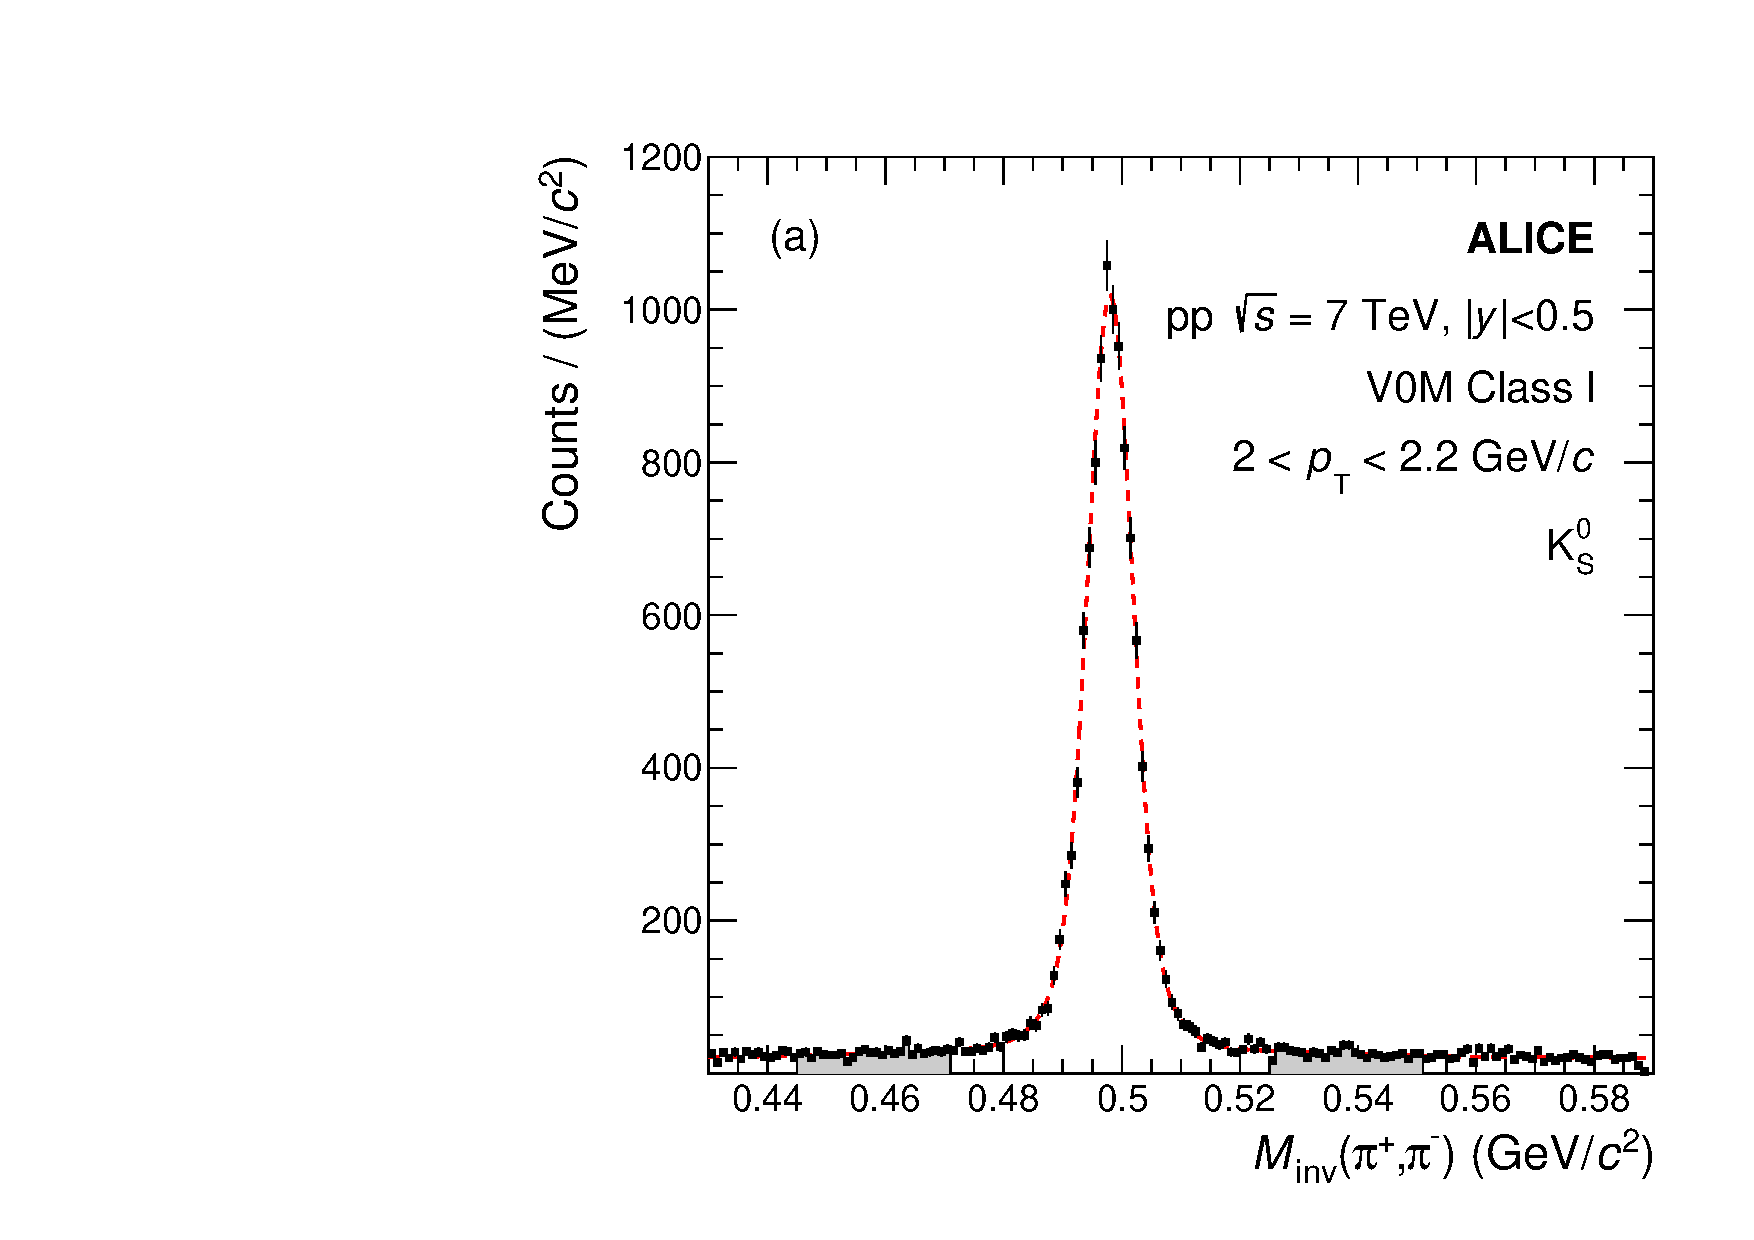
\includegraphics[width=8cm,height=8cm]{figures/InvMass_K0S_I.pdf}
  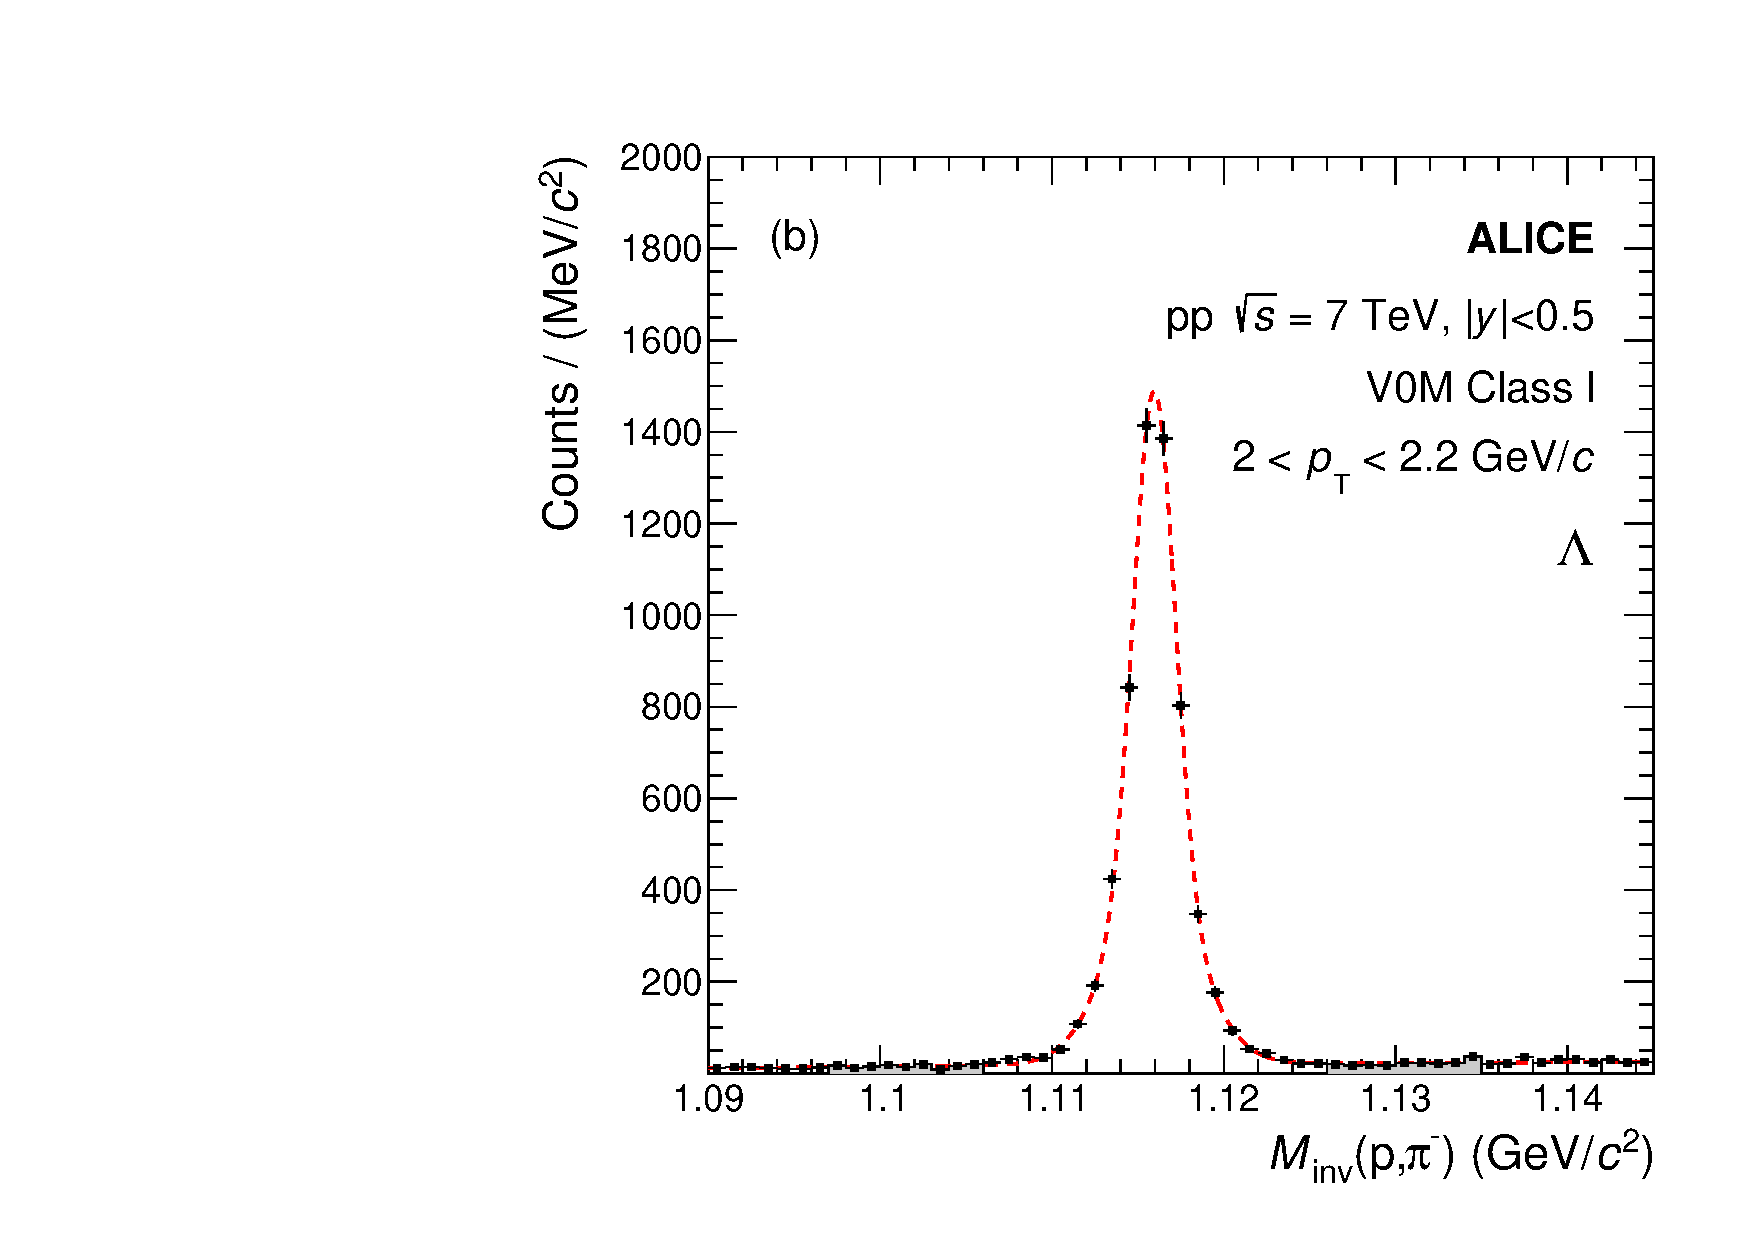
\includegraphics[width=8cm,height=8cm]{figures/InvMass_Lambda_I.pdf}
  \\
  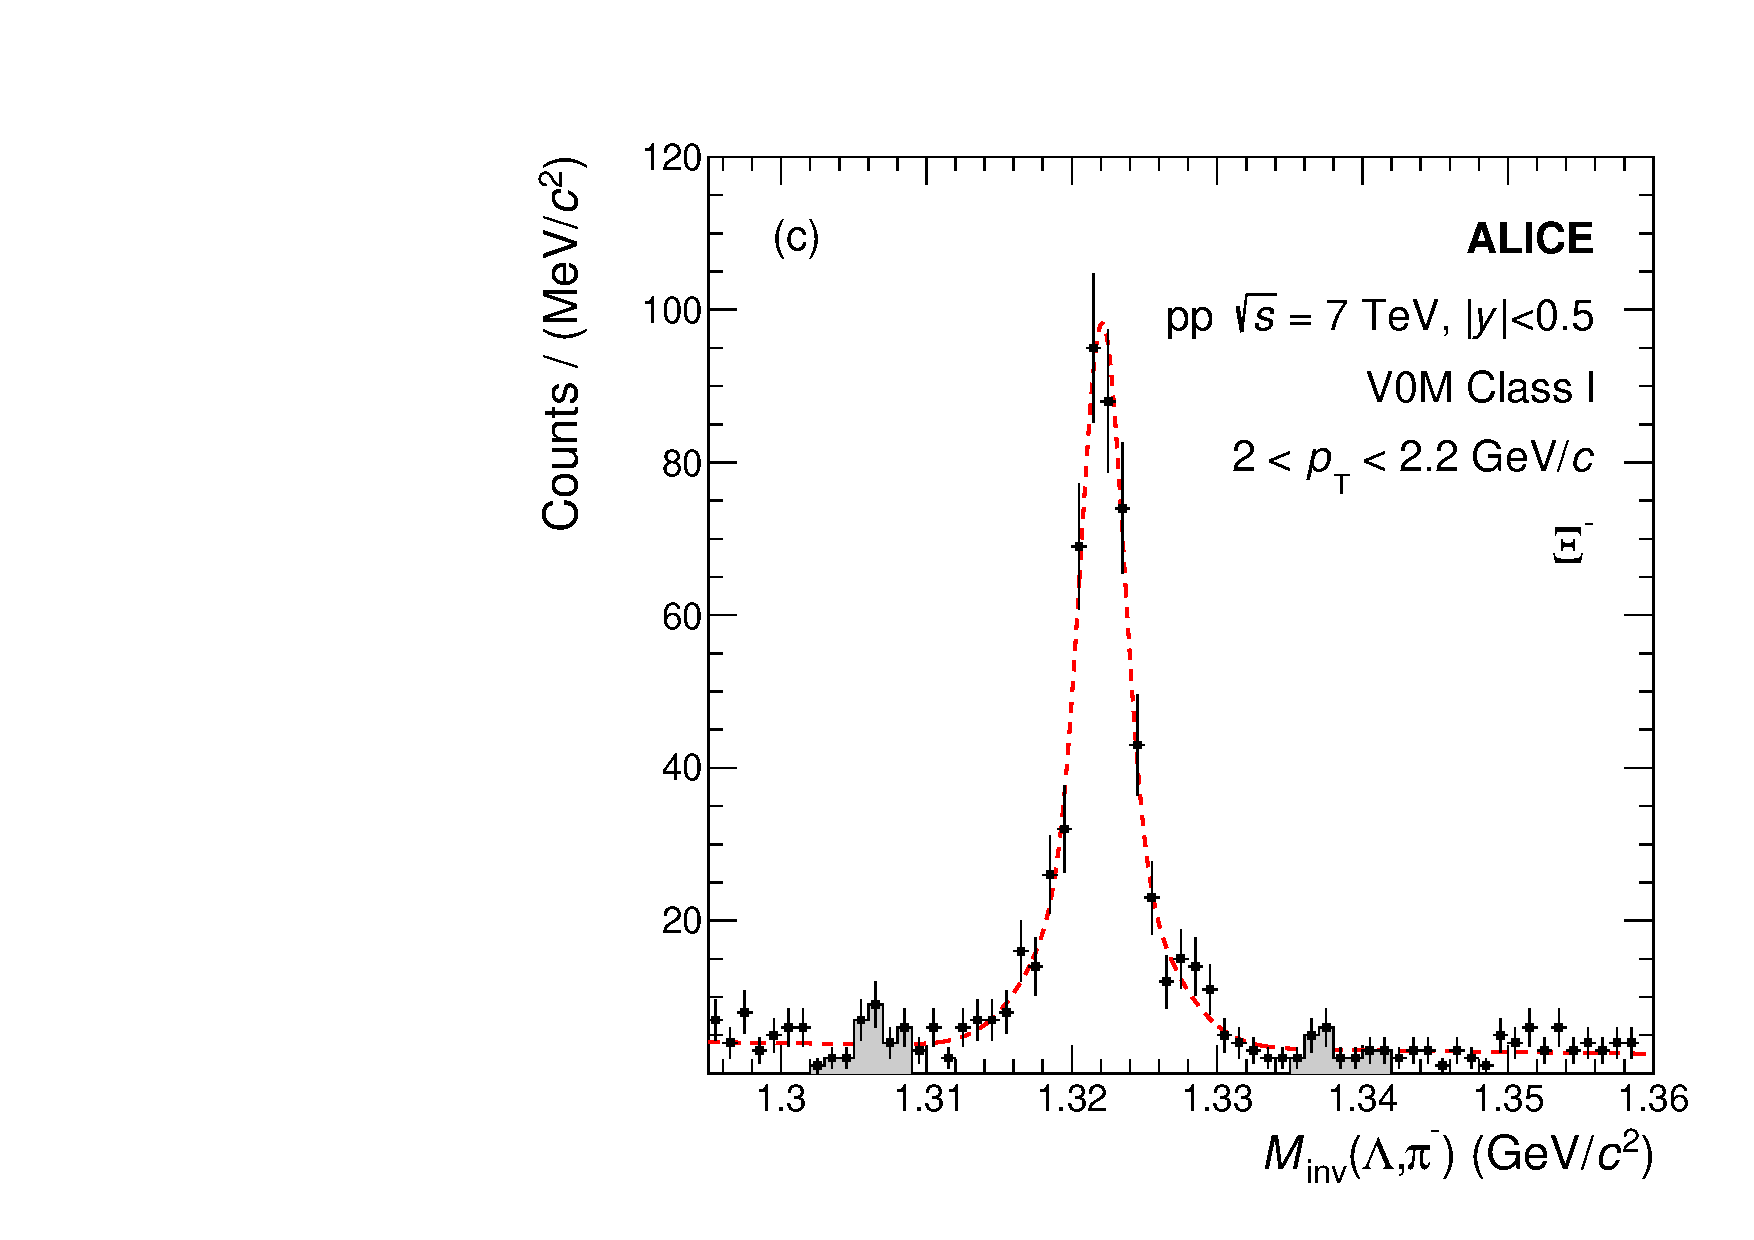
\includegraphics[width=8cm,height=8cm]{figures/InvMass_Xi_I.pdf}
  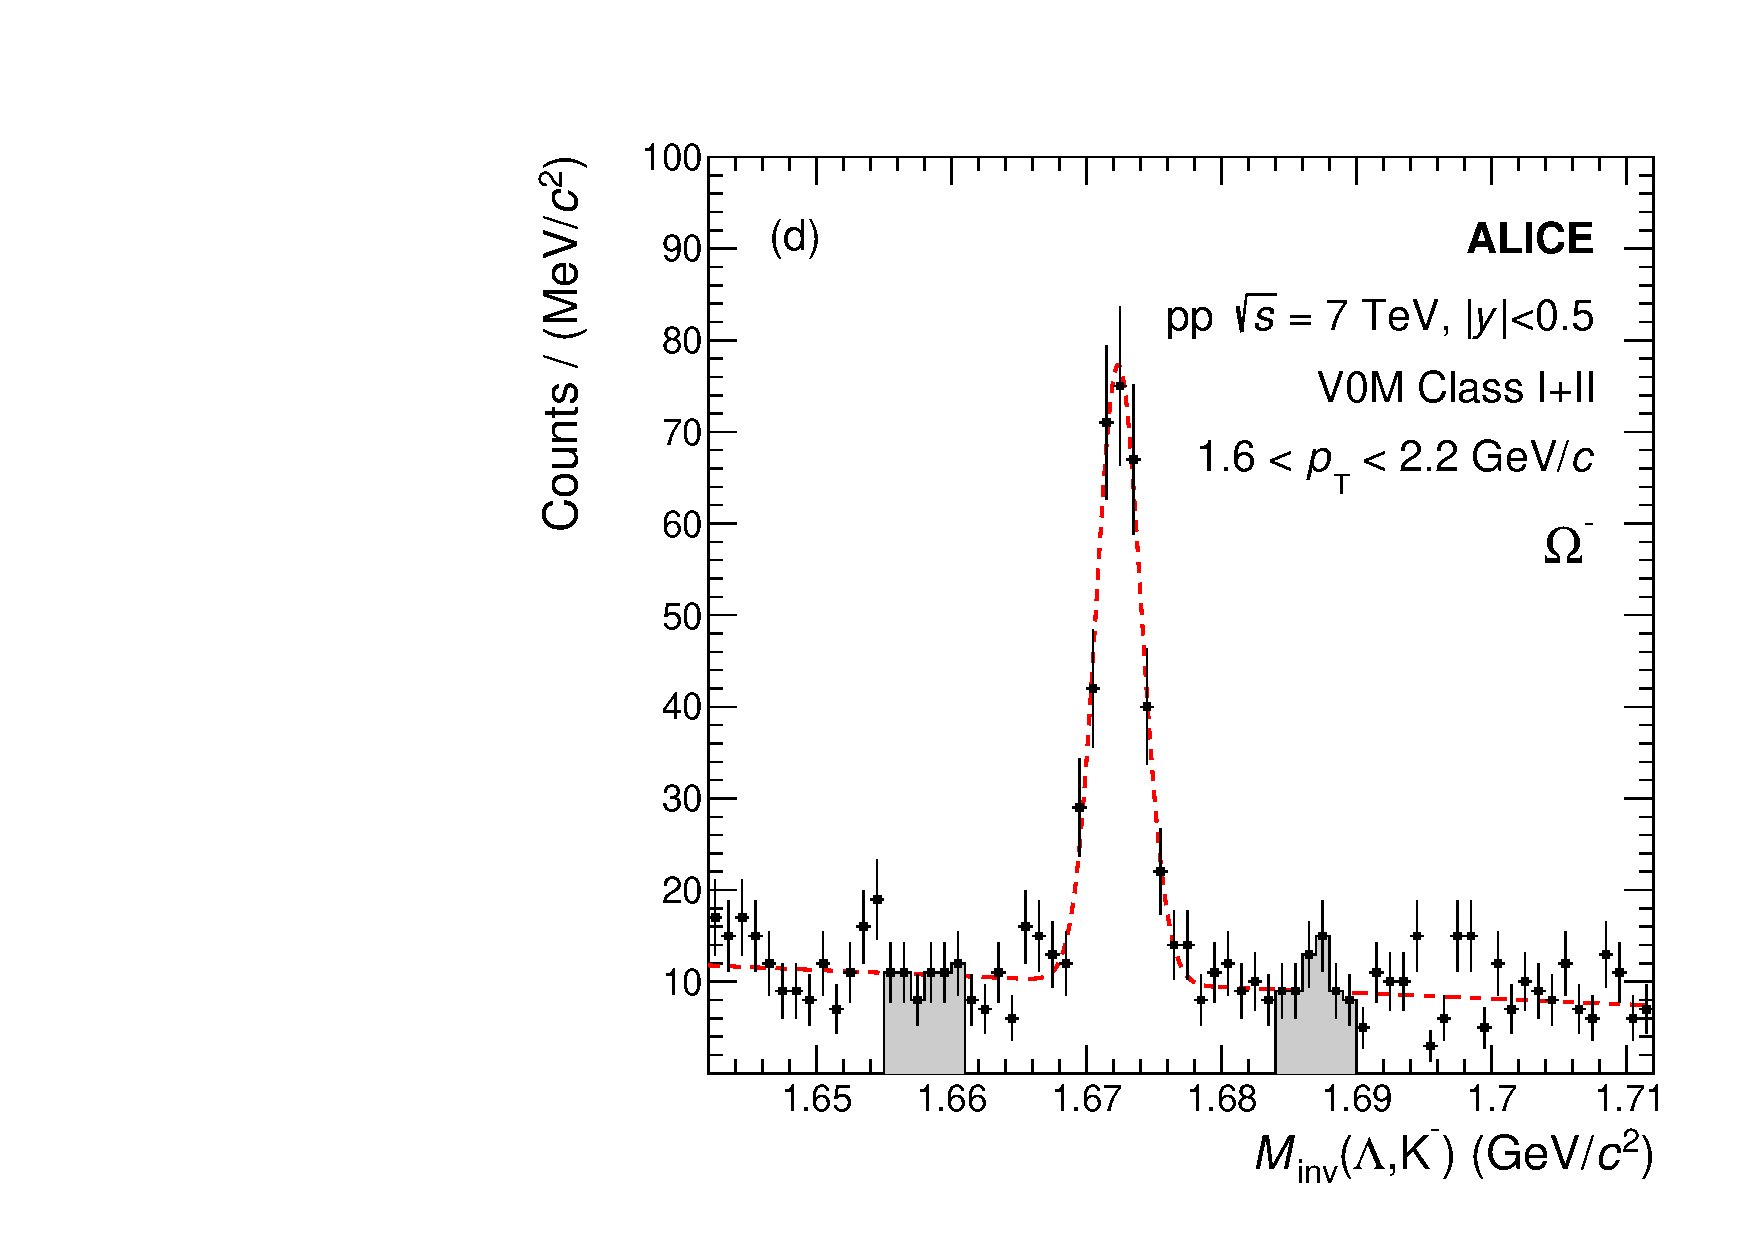
\includegraphics[width=8cm,height=8cm]{figures/InvMass_Omega_I_II.pdf}
  \caption{Invariant-mass distributions of (a) \kzero, (b) \lmb, (c) \X\ and (d) \Om\ (bottom right)  decay candidates in selected
    \pt\ ranges for the corresponding highest V0M event multiplicity classes in pp collisions at $\sqrt{s}$ = 7 TeV. The statistical uncertainties are shown by error bars
    and the shaded bands on the sides of the peak represent the regions used to estimate the background. The red dashed curves represent fits using a gaussian 
    peak and a linear background.}
  \label{fig:V0CascSig}
\end{figure*}

\afterpage{\clearpage}

Approximately 20\% of the measured \lmb\ (\almb) signals are from \X\ (\Ix) and $\Xi^{0}$ ($\overline{\Xi}^{0}$)
decays. These feed-down contributions were subtracted using a data-driven approach in which the measured
\X\ (\Ix) spectra are used as input and a simulation is used to evaluate the fraction of reconstructed 
\lmb\ (\almb) coming from \X\ (\Ix) decays. Since production rates of $\Xi^{0}$ and $\overline{\Xi}^{0}$
 have not been measured, their contribution is estimated by assuming that they are as abundant as their
charged counterparts and that their momentum distributions are identical. 

Because in the specific case of the cascade analysis the measurement is performed in large momentum 
intervals because of the limited amount of data, efficiencies are reweighted in each \pt\ bin to take into 
account differences between generated and real data spectral shapes. 

Systematic uncertainties for \kzero, \lmb, \almb, \X, \Ix, \Om\ and \Mo\ are estimated following the 
procedure described in~\cite{Abelev:2013haa,  Adam:2015vsf}. The main sources of systematic 
uncertainty in these measurements are track selections (up to $\sim$6\%), knowledge of detector 
materials (4\%), feed-down from \X\ (\Ix) and $\Xi^{0}$ ($\overline{\Xi}^{0}$) for the \lmb\ (\almb) (up to $\sim$4\%) 
and topological selections, which contribute with a $\sim$1-8\% uncertainty. 
The contributions to 
systematic uncertainties are summarized in Tab.~\ref{tab:sysweakdecay}. As in previous work, 
the study of systematic uncertainties was repeated for all event classes to determine
differences in how each contribution affects results from each of these classes. 

\begin{table*}[ph!]
  \begin{tabularx}{\linewidth}{l*{3}{Y}*{3}{Y}}
\hline\hline
    Hadron species &  \multicolumn{3}{c}{\kzero} & \multicolumn{3}{c}{\lmb(\almb)} \\
    \pt\ range (\GeVc)                    &  0.05 & 6.2 & 11.0 &   0.5 & 3.7 & 7.2 \\
    \cmidrule(lr){2-4} \cmidrule(lr){5-7} 
    Material budget                 &   4.0 & 4.0 & 4.0  &   4.0 & 4.0 & 4.0 \\
    Transport code & \multicolumn{3}{c}{negligible}  &   1.0 & 1.0 & 1.0 \\
    Track selection                 &   1.0 & 5.0 & 0.8  &   0.2 & 5.9 & 4.3 \\ 
    Topological selection           &   2.6 & 1.1 & 2.3  &   0.8 & 0.6 & 3.2 \\ 
    Particle identification         &   0.1 & 0.1 & 0.1  &   0.2 & 0.2 & 3.0 \\ 
    Efficiency determination        &   2.0 & 2.0 & 2.0  &   2.0 & 2.0 & 2.0 \\
    Signal extraction               &   1.5 & 1.2 & 3.6  &   0.6 & 0.7 & 3.0 \\
    Proper lifetime                 &   1.3 & 0.1 & 0.2  &   0.3 & 2.3 & 0.1 \\
    Competing decay rejection       & negl. & 0.7 & 1.3  & negl. & 1.0 & 6.2 \\
%    Competing V$^{0}$ Rejection   &   -- & 0.7 & 1.3   &   -- & 1.0 & 6.5   \\
%    Competing \sXi Rejection   &   \multicolumn{3}{c}{--}   &   \multicolumn{3}{c}{--}  \\
    Feed-down correction & \multicolumn{3}{c}{not applicable}   &   3.3 & 2.1 & 4.3   \\
    \cmidrule(lr){2-4} \cmidrule(lr){5-7} 
    Total                           &   5.6 & 6.9 & 6.4  &   5.8 & 8.2 & 11.2 \\ 
    Common ($N_{ch}$-independent)   &   5.0 & 5.9 & 4.4  &   5.4 & 7.8 & 9.9  \\ 
\hline\hline
    Hadron species & \multicolumn{3}{c}{\X(\Ix)} & \multicolumn{3}{c}{\Om(\Mo)} \\
    \pt\ range (\GeVc)                    &   0.8 & 2.1 & 5.8   &   1.2 & 2.8 & 4.7 \\
    \cmidrule(lr){2-4} \cmidrule(lr){5-7} 
    Material budget                 &   4.0 & 4.0 & 4.0  &   4.0 & 4.0 & 4.0 \\
    Transport code                  &   1.0 & 1.0 & 1.0  &   1.0 & 1.0 & 1.0 \\
    Track selection                 &   0.4 & 0.3 & 2.2  &   0.8 & 0.6 & 4.1 \\ 
    Topological selection           &   3.1 & 2.0 & 4.0  &   5.0 & 5.6 & 8.1 \\ 
    Particle identification         &   1.0 & 0.2 & 1.2  &   1.1 & 1.7 & 3.2 \\ 
    Efficiency determination        &   2.0 & 2.0 & 2.0  &   2.0 & 2.0 & 2.0 \\
    Signal extraction               &   1.5 & 0.2 & 1.0  &   3.2 & 2.5 & 2.3 \\
    Proper lifetime                 &   0.9 & 0.1 & 0.1  &   2.2 & 0.7 & 0.7 \\
    Competing decay rejection   &  \multicolumn{3}{c}{not applicable}  &  0.2 & 4.2 & 5.2 \\
%    Competing V$^{0}$ Rejection   & \multicolumn{3}{c}{--}  & \multicolumn{3}{c}{--}  \\
%    Competing \sXi Rejection   &  \multicolumn{3}{c}{--}  &  0.2 & 4.2 & 5.2 \\
    Feed-down correction & \multicolumn{3}{c}{negligible}  &  \multicolumn{3}{c}{negligible} \\
    \cmidrule(lr){2-4} \cmidrule(lr){5-7} 
    Total                           &   5.9 & 5.0 & 6.7  &   7.9 & 9.0 & 12.1 \\ 
    Total ($N_{ch}$-independent)   &   5.2 & 4.5 & 6.2  &   7.3 & 8.7 & 11.6 \\ 
\hline\hline
  \end{tabularx}
  ~\newline
    \caption{Main sources and values of the relative systematic uncertainties (expressed in \%) of the \pt-differential yields of \kzero, \lmb(\almb), \X(\Ix) and \Om(\Mo). The values are reported for low, intermediate and high \pt. The contributions that act differently in the various event classes are removed from the Total (quadratic sum of all contributions), defining the $N_{ch}$-independent ones, which are correlated across different multiplicity intervals.}
  \label{tab:sysweakdecay}  
\end{table*}



